%\subsection{Workflow}
\label{sec:workflow}


\begin{figure}
\centering
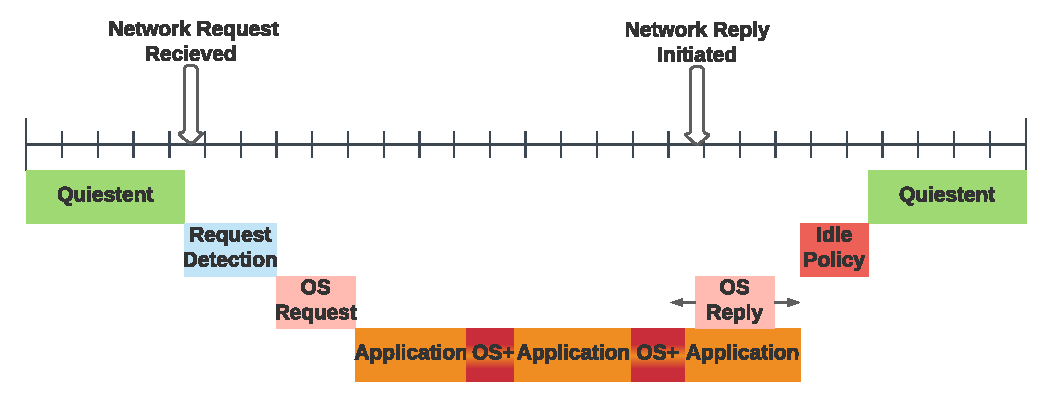
\includegraphics[width=0.5\textwidth]{figures/timeline_chart}
\caption[]{W timeline for a single application request}
\label{fig:timeline}
\end{figure}

From an OS perspective we break down network driven processing into stages that allows us to organize and reflect the OS and application interaction with the workload request timeline.  This break down is illustrated in figure~\ref{fig:timeline}.   

\subsection{Quiescent}
Given the packet and transactional nature of network driven services a quiescent period, in which no request is present at the server, precedes activity on the server. 

\subsubsection{Open Loop:}
In an open loop scenario like a Memcached workload, the external request rate induces an inter-arrival gap that will drive the quiescent period -- longer at lighter loads (lower queries per second (QPS)) and shorter a heavier loads (higher QPS). Largely the arrival rate can be considered independent of the time required to service a request.  A systems performance is typically evaluated in terms of 99\% tail latency it achieves.  Moreover, providers often set a Quality of Service (QoS), such as  a 99\% tail latency of 500${\mu}$s.  As Mootaz et al. observed, that in latency focused workloads, the "latency-slack" between the mean time to servicing a request and the QoS target creates an opportunity for energy-performance tradeoffs.  In particular, it maybe possible to reduce mean performance by not complete all requests as fast as possible or processing immediately upon a request arrival and reduce energy consumption while not violating the QoS target.  

\subsubsection{Closed Loop:}
In a closed loop setting, like snapshotting a database to a remote server or video streaming, the arrival rate of the next request, that forms the overall task, depends on how long it takes to service the current request.  However, the quiescent period is bounded by the network round trip time, that depends on  the size of a request and reply packets, and the remote processing time.   System performance is largely evaluated on how fast a server can complete the entire task given a network link speed and remote system.  Given workload specific characteristics the processing required and round-trip costs it is possible, as we will see, to find configurations in which the OS interacts with slowing down to improve both time and energy.   Often research tends to categorize close loop settings as either not representative of cloud computing or imply that energy-performance tradeoffs are not interesting due to the hight utilization it implies.  

Given our goal of studying and explaining the implications of the OS on network driven processing our analysis framework and evaluation includes closed loop settings.  In particular, we use a simple ping-pong application to stress OS behavior while varying packet-sizes to reveal how OS path length and path efficiency interacts with slowing down relative to the time to process a request versus the network time.  Additionally we use a second closed loop that stresses single core application processing with negligible packet sizes to evaluate if OS structure can impact the application efficiency.  

 
\subsection{OS Request Detection}

Fundamental to any operating system is how it detects and schedule processing in response to IO device activity.  At the two extremes are interrupt and poll driven detection.  

\subsubsection{Interrupt driven IO}
Using interrupts has three important implications: 1) Interrupts can be used to transition a processor from a halted state in which the OS entered to sleep the processor (at some selected HW sleep state (C-state)) in response to external activity, 2)  Interrupts allow an OS to arbitrate processing across competitive devices and processing in a general multi-programmed multi-device setting, 3) interrupt processing has an inherent performance costs associated with it -- in terms of latency in starting handling of an in-bound request, either because of the costs associated with preempting currently scheduled work\cite{intelpaper} or exit penalties associated with the C-state that the processors is halted in\cite{}.  Interrupt processing can also have a negative impact on the instruction efficiency, measured in Instructions Per Cycle (IPC), due to induced micro-architecture hazards such as the inability to prefetch or speculatively execute across an interrupt.

\subsubsection{Poll driven IO}

Most modern devices expose a memory, if not cache, friendly mechanism, that permits the processors to read a per-core memory address to determine if the device, such as the Network Interface Card (NIC) has received data that requires processing by the core.  This facility allows software to directly poll the device and initiate software handling without an interrupt.  This approach reduces latency and other performance penalties associated with interrupt driven IO.  However, the rate a which the device is checked requires active CPU activity limiting the ability to halt the cores when there is not work to be done.  In the extreme, a customized OS supporting a single application can run a poll loop on every core to constantly check for work, conduct the work and then go back to polling for new work and thus never halting the processors due to idleness.   While used in a slightly different context to Kim et al.\cite{hank} we will refer to this regime as 'no-idle' as it results in a similar energy management strategy albeit in the context of network driven processing.  In general such an aggressive poll approach is assumed to maximize performance by minimizing latency and avoid interrupts overheads.

\subsubsection{Hybrid driven IO}

A general purpose operating system typically exploits some form of hybrid alternating between using interrupts for device and polling the device for some period before switching back to using interrupts for the device.  A general purpose   

Linux has a complex, 

\subsubsection{Interrupt Delaying}

 

In order to help seed the context of how slowing down processor frequency and ITR-Delay can affect an application's performance and energy, figure~\ref{fig:timeline} presents a generalized breakdown of components along a typical packet receive path. We believe this modeling is applicable across different OS structures and networking hardware's as it details a set of fundamental components that all packet processing frameworks must undergo.

%\subsection{Application Perspective}
%Figure~\ref{fig:timeline} shows the application is waiting to be woken up to process new packets (a). Next, an interrupt (b) is fired and the OS network stack begins processing the received packet (c). The application level work begins, alongside there are also interspersed OS work which may or may not be in direct support of application(d). The tail end of the application work (e) typically entails a response packet being sent, the period of time with which the response packet is physically sent can proceed in parallel with the rest of the application level work. The end of every request handling (f) also revolves a set of OS policies to decide the next state of the software and hardware. Work is time spent executing instructions required to service a request, it is a function of the software, hardware, and workload itself. Whereas, idle time is a function of arrival rate of packets.
%
%\subsection{Hardware Perspective}
%Slowing down of the processor causes an increase in the time spent in portions of application and OS work while reducing energy use. Slowing down of interrupt delays contributes to the increase of time spent in the idle states, the longer a processor idles the more energy it can save.
%
%\subsection{OS Perspective}
%OSes overall behaviour is a function of how it behaves during both the working and idle portions of time, there also exists a clear inter-relationship between the two. 
%
%The amount of energy used during this idle period is dependent upon the OS idling policies; in terms of which level of idle state is selected.
%
\subsection{Equations}

%\subsection{ITR-Delay algorithm}
